\section{Experiments}

\subsection{Dataset and Evaluation Methods}
The dataset used in our experiments is provided by StackOverflow.com. Currently, there are 2.2 million questions, 4.8 millions answers, over 35 thousands tags in this dataset\cite{DataDump}.

We prepared 1,050,000 posts (a post is either a question or an answer)  as the training data $S_{train}$. Also we randomly sampled 5 groups of test data, each with 1000 posts.$S_{test}^i, i \in [1, 5]$.

In our experiments, precision and recall are the metrics to evaluation the predicted results. Here is the definition of the \emph{precision} and \emph{recall}:
$$ \text{Precision}=\frac{tp}{tp+fp}, \text{Recall}=\frac{tp}{tp+fn} $$
where $tp$ is the number of true positive samples, $fp$ is the number of false positive samples and $fn$ is the number of false negative samples.

As we mentioned in \emph{Introduction}, the big challenge of tag prediction is that tags are often quite subjective and incomplete. As a result, it will be problematic to conclude that a tag is ``correctly" predicted only when it appears in user-defined tags. For example, if a question is tagged with ``java" but predicted tag is ``jdk", we still believe it is a \emph{"good"} prediction because in real life, ``jdk" is closed related with ``java".

Thus, instead of measure the ``goodness" of a tag with only \emph{match/unmatch}, we assign each predicted tag with a relevance score $s, s \in [0, 1]$. The higher the score, the more
relevant two tags are.

To get the relevance score $s$, we proposed an evaluation method which makes use of the Kullback–Leibler divergence(a.k.a. KL-distance). KL-distance is an asymmetric measure of the difference between two probability distributions $P$ and $Q$. In our case, each tag has a corresponding \emph{word distribution} and we assume that similar tags will often have similar word distribution. Note that although $KL(P, Q)$ and $KL(Q, P)$ is asymmetrical, in practical, the value of
$KL(Q, P)$ and $KL(P, Q)$ is often very close.

Also, in our experiments, We are interested in the impact of the number $N$ of the predicted tags. We will measure the how the precision/recall changes as $N$ varies.

\subsection{Experimental Results}
\subsubsection{Naive Bayes}
Table \ref{tb:nbresult} demonstrates the prediction results with different numbers of predicted tags. We can see that the recall increases as $N$ goes up; whereas the precision drops when $N$ increases.

In figure \ref{fig:naive}, we can see the difference between Naive Bayes model with and without re-ranking. The significant improvement in both precision and recall proves the effectiveness of the re-ranking.

\begin{figure}[htb!]
\centering%
    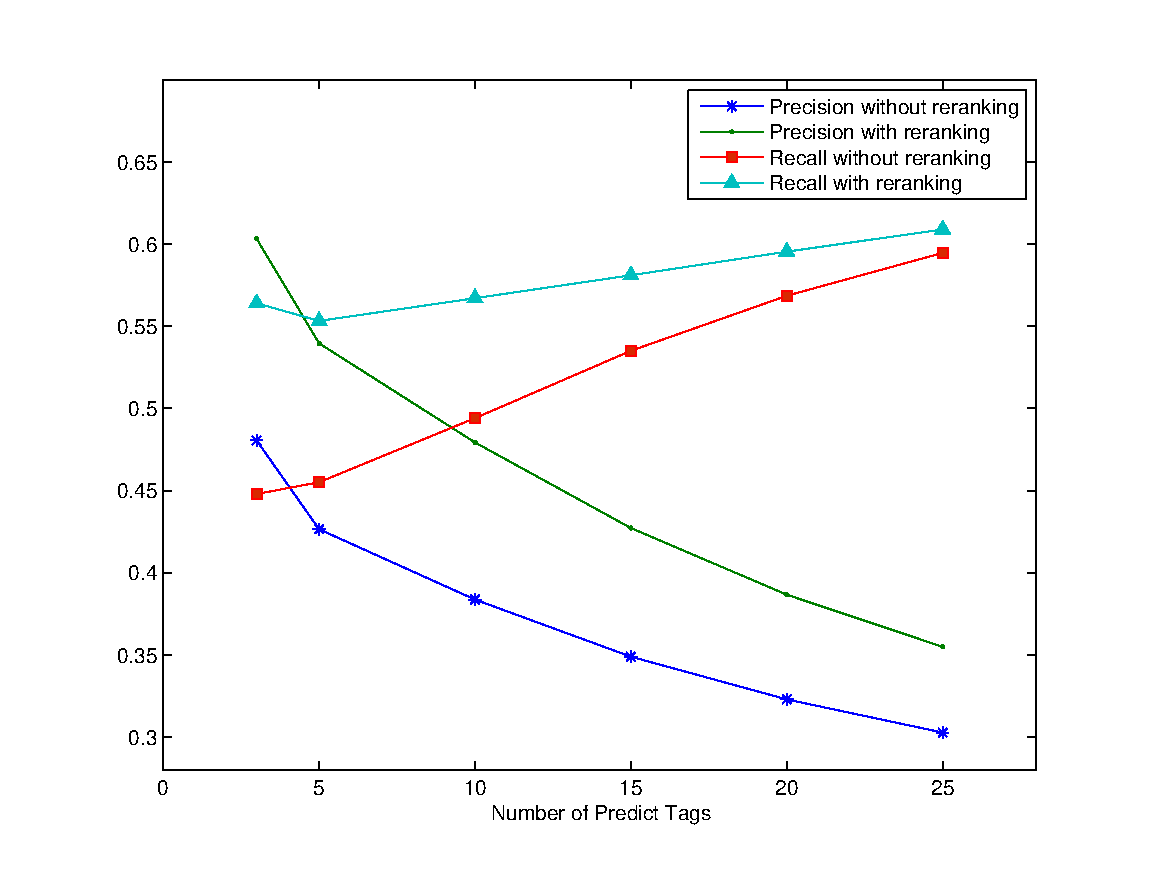
\includegraphics[scale=0.60]{pic/nb_result.eps}
\caption{Performance of Naive Bayes Classifier: with and without re-ranking}
\label{fig:naive}
\end{figure}

\begin{table}
\centering \caption{\label{tb:nbresult}Result of Naive Bayes(with re-ranking)}
\begin{tabular}{l|l|l|l|l|l|l|l}
	\hline Test Set & Size & 3 & 5 & 10 & 15 & 20 & 25 \\
	\hline \multirow{2}{*}{$D_1$} & Precision & 0.6430 & 0.5652 & 0.5052 & 0.4467 & 0.4014 & 0.3666 \\
	\cline{2-8} & Recall & 0.5851 & 0.5471 & 0.5598 & 0.5738 & 0.5877 & 0.6021 \\
	
	\hline \multirow{2}{*}{$D_2$} & Precision & 0.6065 & 0.5517 & 0.4904 & 0.4359 & 0.3931 & 0.3603 \\
	\cline{2-8} & Recall & 0.5897 & 0.5616 & 0.5691 & 0.5807 & 0.5931 & 0.6072 \\
	
	\hline \multirow{2}{*}{$D_3$} & Precision & 0.6084 & 0.5404 & 0.4801 & 0.4282 & 0.3877 & 0.3556å \\
	\cline{2-8} & Recall & 0.5658 & 0.5564 & 0.5709 & 0.5846 & 0.5996 & 0.6121 \\
	
	\hline \multirow{2}{*}{$D_4$} & Precision & 0.5929 & 0.5271 & 0.4669 & 0.4176 & 0.3793 & 0.3491 \\
	\cline{2-8} & Recall & 0.5523 & 0.5541 & 0.5701 & 0.5846 & 0.5990 & 0.6121 \\
	
	\hline \multirow{2}{*}{$D_5$} & Precision & 0.5658 & 0.5141 & 0.4541 & 0.4078 & 0.3720 & 0.3431 \\
	\cline{2-8} & Recall & 0.5276 & 0.5474 & 0.5656 & 0.5814 & 0.5977 & 0.6113 \\
	
	\hline \multirow{2}{*}{Average} & Precision & 0.6033 & 0.5397 & 0.4793 & 0.4272 & 0.3867 & 0.3549 \\
	\cline{2-8} & Recall & 0.5641 & 0.5533 & 0.5671 & 0.5810 & 0.5954 & 0.6090 \\
	
	\hline
\end{tabular}
\end{table}


\subsubsection{K Nearest Neighbors}
Table \ref{tb:nbresult} demonstrates the prediction results with different numbers of predicted tags.

We compared the experimental results in figure \ref{fig:knn} of knn classifier with different $k$, and found that when $k=70$ we can get an optimal recall/precision.

\begin{figure}[htb!]
\centering%
    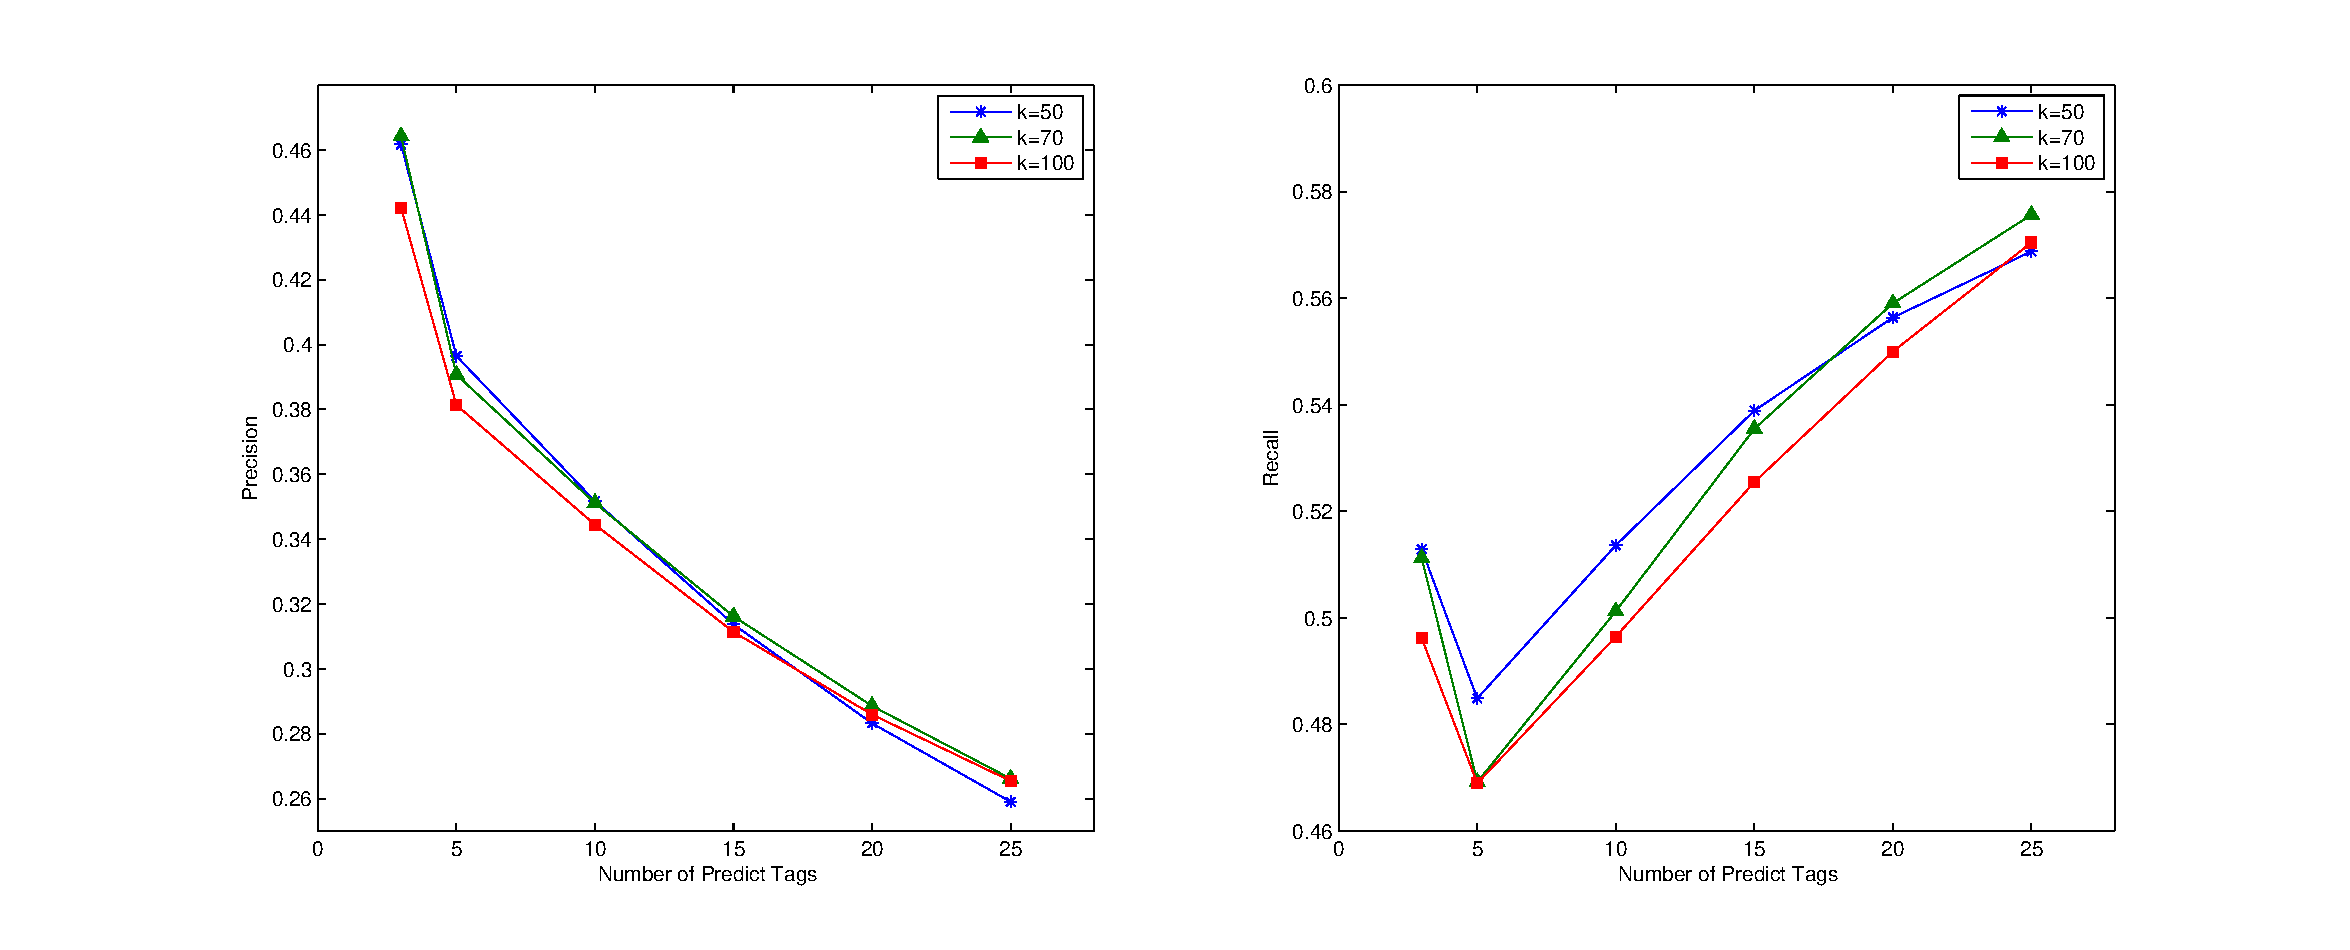
\includegraphics[scale=0.40]{pic/knn}
\caption{Performance of k-NN Classifiers: with different $k$}
\label{fig:knn}

\end{figure}
\begin{table}
\centering \caption{\label{tb:nbresult}Result of KNearest Neighbors(k=70)}
\begin{tabular}{l|l|l|l|l|l|l|l}
	\hline Test Set & Size & 3 & 5 & 10 & 15 & 20 & 25 \\
	\hline \multirow{2}{*}{$D_1$} & Precision & 0.5631 & 0.4168 & 0.3715 & 0.3310 & 0.3001 & 0.2753\\
	\cline{2-8} & Recall & 0.5681 & 0.4638 & 0.4857 & 0.5227 & 0.5503 & 0.5689\\
	
	\hline \multirow{2}{*}{$D_2$} & Precision & 0.4716 & 0.3974 & 0.3578 & 0.3223 & 0.2932 & 0.2700\\
	\cline{2-8} & Recall & 0.5711 & 0.4810 & 0.4983 & 0.5341 & 0.5578 & 0.5751\\
	
	\hline \multirow{2}{*}{$D_3$} & Precision & 0.4742 & 0.3959 & 0.3539 & 0.3176 & 0.2896 & 0.2668 \\
	\cline{2-8} & Recall &0.5287 & 0.4772 & 0.5090 & 0.5401 & 0.5632 & 0.5790\\
	
	\hline \multirow{2}{*}{$D_4$} & Precision &0.4047 & 0.3722 & 0.3389 & 0.3077 & 0.2822 & 0.2611\\
	\cline{2-8} & Recall &0.4521 & 0.4628 & 0.5066 & 0.5410 & 0.5631 & 0.5784 \\
	
	\hline \multirow{2}{*}{$D_5$} & Precision &0.4074 & 0.3712 & 0.3332 & 0.3023 & 0.2775 & 0.2573 \\
	\cline{2-8} & Recall & 0.4358 & 0.4609 & 0.5063 & 0.5392 & 0.5608 & 0.5767\\
	
	\hline \multirow{2}{*}{Average} & Precision & 0.4642 & 0.3907 & 0.3511 & 0.3162 & 0.2885 & 0.2661\\
	\cline{2-8} & Recall &0.5112 & 0.4691 & 0.5012 & 0.5354 & 0.5590 & 0.5756\\
	
	\hline
\end{tabular}
\end{table}

\subsubsection{Simple Match}
Table \ref{tb:nbresult} demonstrates the prediction results with different numbers of predicted tags. As the results suggest, although the simple match approach is quite simple, its performance is still acceptable.

\begin{table}
\centering \caption{\label{tb:nbresult}Result of Simple Match}
\begin{tabular}{l|l|l|l|l|l|l|l}
	\hline Test Set & Size & 3 & 5 & 10 & 15 & 20 & 25 \\
	\hline \multirow{2}{*}{$D_1$} & Precision & 0.2143 & 0.2069 & 0.1855 & 0.1626 & 0.1451 & 0.1324\\
	\cline{2-8} & Recall & 0.2808 & 0.2944 & 0.3185 & 0.3466 & 0.3699 & 0.3907\\
	
	\hline \multirow{2}{*}{$D_2$} & Precision & 0.2172 & 0.2027 & 0.1801 & 0.1586 & 0.1423 & 0.1303\\
	\cline{2-8} & Recall &0.2854 & 0.3009 & 0.3261 & 0.3525 & 0.3754 & 0.3955\\
	
	\hline \multirow{2}{*}{$D_3$} & Precision &0.2146 & 0.1981 & 0.1749 & 0.1547 & 0.1395 & 0.1283\\
	\cline{2-8} & Recall & 0.2844 & 0.3047 & 0.3310 & 0.3567 & 0.3794 & 0.3993\\
	
	\hline \multirow{2}{*}{$D_4$} & Precision & 0.2127 & 0.1946 & 0.1706 & 0.1513 & 0.1369 & 0.1264\\
	\cline{2-8} & Recall & 0.2852 & 0.3077 & 0.3359 & 0.3610 & 0.3828 & 0.4027\\
	
	\hline \multirow{2}{*}{$D_5$} & Precision &0.2140 & 0.1922 & 0.1671 & 0.1483 & 0.0810 & 0.1247\\
	\cline{2-8} & Recall &0.2874 & 0.3110 & 0.3406 & 0.3654 & 0.3866 & 0.4065\\
	
	\hline \multirow{2}{*}{Average} & Precision & 0.2146 & 0.1989 & 0.1756 & 0.1551 & 0.1397 & 0.1284\\
	\cline{2-8} & Recall &0.2846 & 0.3037 & 0.3304 & 0.3564 & 0.3788 & 0.3990\\
	
	\hline
\end{tabular}
\end{table}

\subsection{Comparison and Conclusion}
\begin{figure}[htb!]
\centering%
    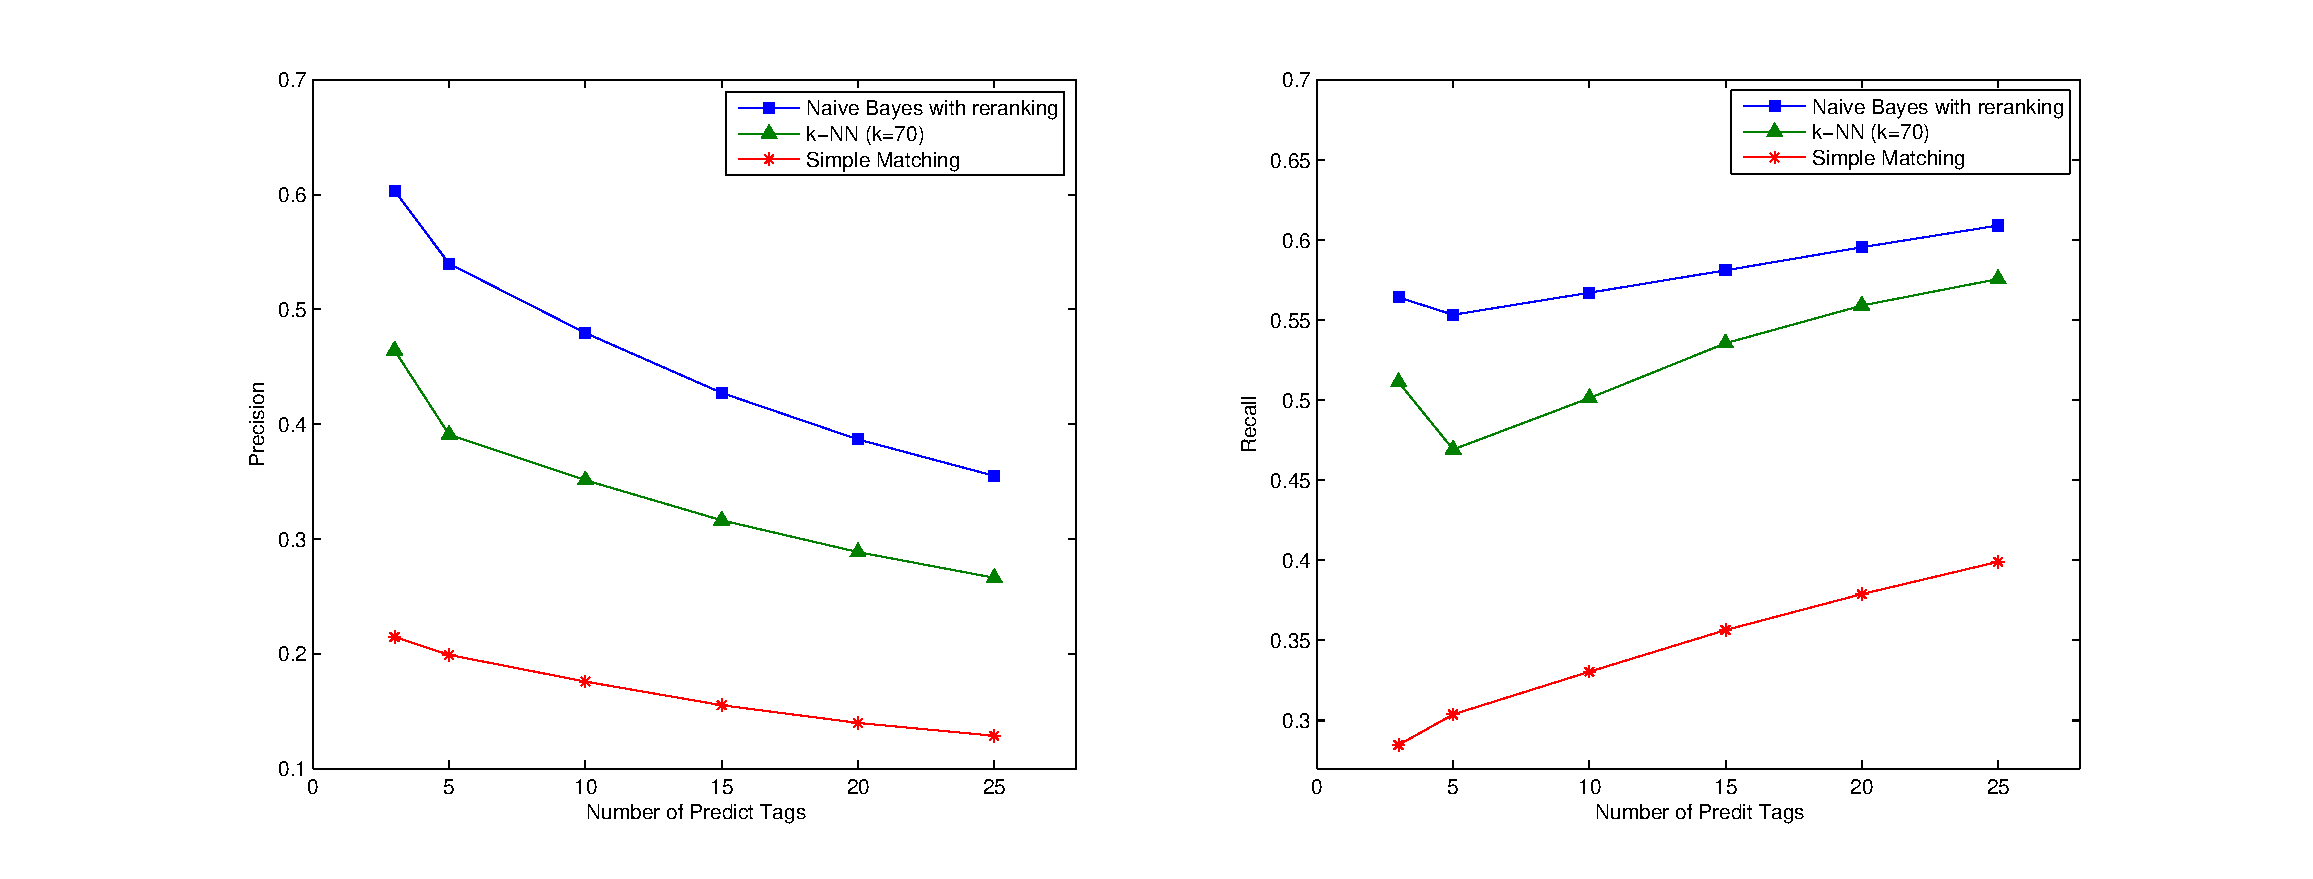
\includegraphics[scale=0.40]{pic/compare}
\caption{Overall comparsion of three proposed methods}
\label{fig:compare}
\end{figure}

Figure \ref{fig:compare} is a comprehensive comparision of all three proposed methods.

From the figure we can see Naive Bayes classifier yields the best precision/recall, with k-NN followed closely. Both of the proposed methods has significantly outperformed the baseline method by over 20\% percent in both recall and precision.

